\documentclass[border=0.5cm]{standalone}

% this is not done yet, takenr from the R library

\usepackage[latin1]{inputenc}
\usepackage{tikz}

%% using the pgf-umlcd package, see https://github.com/xuyuan/pgf-umlcd
\usepackage{pgf-umlcd} 
%\usetikzlibrary{shapes,arrows, positioning, decorations.markings}

\renewcommand{\umlfillcolor}{blue!10}
\renewcommand{\umldrawcolor}{black}

\begin{document}
\pagestyle{empty}


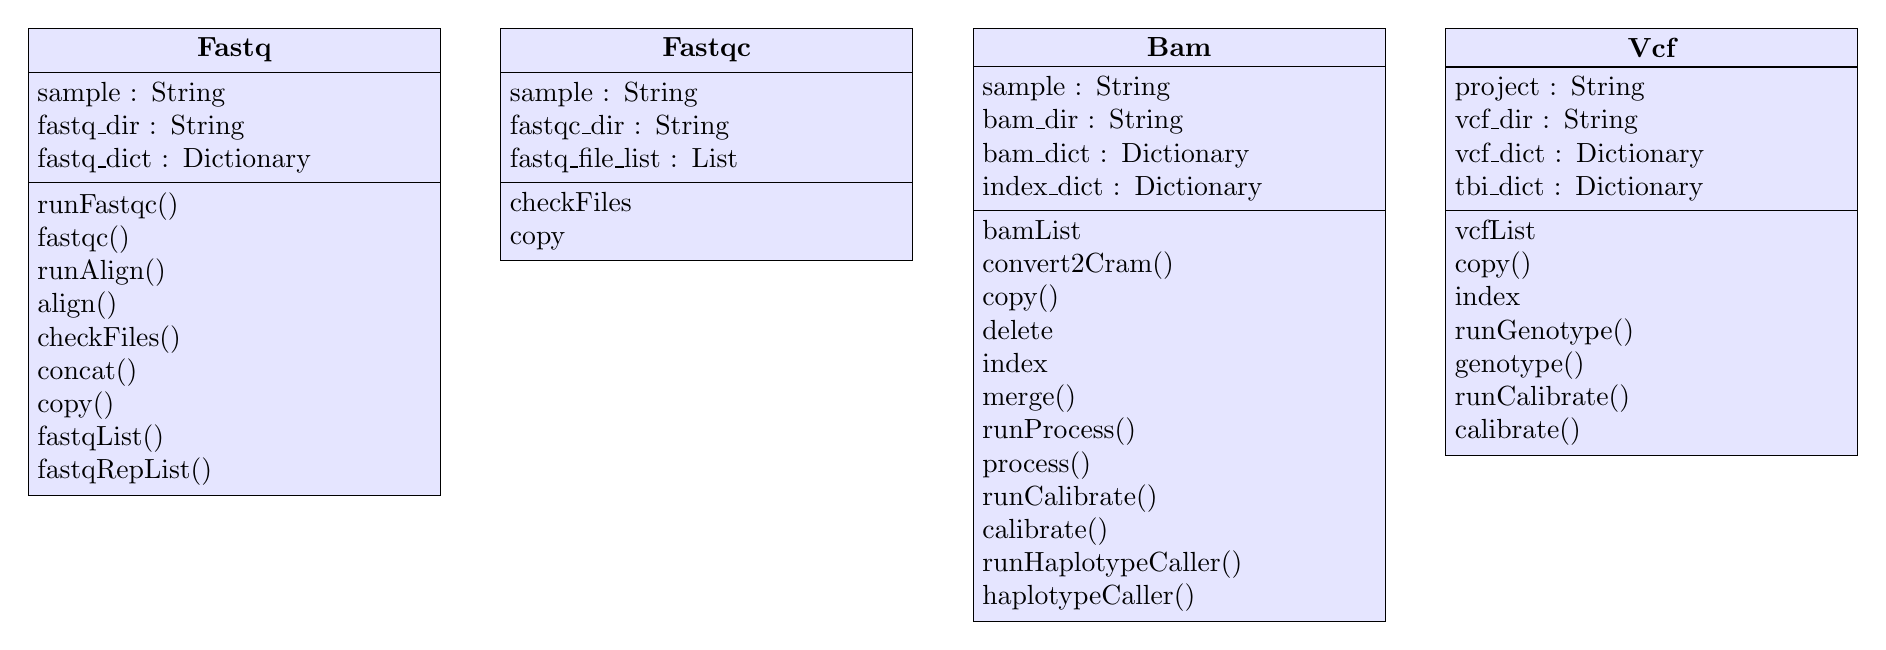
\begin{tikzpicture}

  \begin{class}[text width=5cm]{Fastq}{0,0}
    \attribute{sample : String}
    \attribute{fastq\_dir : String}
    \attribute{fastq\_dict : Dictionary}
    %\attribute{balance : Dollars = 0}
    \operation{runFastqc()}
    \operation{fastqc()}
    \operation{runAlign()}
    \operation{align()}
    \operation{checkFiles()}
    \operation{concat()}
    \operation{copy()}
    \operation{fastqList()}
    \operation{fastqRepList()}
  \end{class}

  \begin{class}[text width=5cm]{Fastqc}{6,0}
    % \inherit{GOSLib}
    \attribute{sample : String}
    \attribute{fastqc\_dir : String}
    \attribute{fastq\_file\_list : List}
    \operation{checkFiles}
    \operation{copy}
  \end{class}

  \begin{class}[text width=5cm]{Bam}{12,0}
    % \inherit{GOSLib}
    \attribute{sample : String}
    \attribute{bam\_dir : String}
    \attribute{bam\_dict : Dictionary}
    \attribute{index\_dict : Dictionary}
    \operation{bamList}
    \operation{convert2Cram()}
    \operation{copy()}
    \operation{delete}
    \operation{index}
    \operation{merge()}

    \operation{runProcess()}    
    \operation{process()}
    \operation{runCalibrate()}
    \operation{calibrate()}
    \operation{runHaplotypeCaller()}
    \operation{haplotypeCaller()}
  \end{class}

  \begin{class}[text width=5cm]{Vcf}{18,0}
    % \inherit{GOSLib}
    \attribute{project : String}
    \attribute{vcf\_dir : String}
    \attribute{vcf\_dict : Dictionary}
    \attribute{tbi\_dict : Dictionary}

    \operation{vcfList}
    \operation{copy()}
    \operation{index}
    \operation{runGenotype()}
    \operation{genotype()}
    \operation{runCalibrate()}
    \operation{calibrate()}
  \end{class}



\end{tikzpicture}

\end{document}

%%% Local Variables:
%%% mode: latex
%%% TeX-master: t
%%% End:
